\item[(d)]
\section{Poles and Zeros, Pole-Zero Map, and ROC}

\subsection*{Problem Statement}
Calculate the poles and zeros of \( H(z) \) and include a sketch of the pole-zero map in your report. Also, include the region of convergence (ROC) in the pole-zero map.

\subsection*{Theoretical Background}
The poles and zeros of a transfer function \( H(z) \) can be found by solving the numerator and denominator equations of \( H(z) \). The poles are the values of \( z \) that make the denominator zero, and the zeros are the values of \( z \) that make the numerator zero.

\subsection*{Mathematical Derivation}
The transfer function derived in the previous task is:
\[ H(z) = \frac{z^2}{z^2 + \frac{1}{15} z - \frac{2}{5}} \]

\subsubsection*{Zeros}
The zeros are the roots of the numerator \( z^2 = 0 \), which gives:
\[ z = 0 \]

\subsubsection*{Poles}
The poles are the roots of the denominator \( z^2 + \frac{1}{15} z - \frac{2}{5} = 0 \).

Using the quadratic formula \( z = \frac{-b \pm \sqrt{b^2 - 4ac}}{2a} \), where \( a = 1 \), \( b = \frac{1}{15} \), and \( c = -\frac{2}{5} \):
\[ z = \frac{-\frac{1}{15} \pm \sqrt{\left( \frac{1}{15} \right)^2 + \frac{8}{5}}}{2} \]
\[ z = \frac{-\frac{1}{15} \pm \sqrt{\frac{1}{225} + \frac{360}{225}}}{2} \]
\[ z = \frac{-\frac{1}{15} \pm \sqrt{\frac{361}{225}}}{2} \]
\[ z = \frac{-\frac{1}{15} \pm \frac{19}{15}}{2} \]
\[ z = \frac{-1 \pm 19}{30} \]
\[ z = \frac{18}{30} = \frac{3}{5}, \quad z = \frac{-20}{30} = -\frac{2}{3} \]

Thus, the poles are at:
\[ z = \frac{3}{5}, \quad z = -\frac{2}{3} \]

\subsection*{Pole-Zero Map}
The pole-zero map illustrates the location of the poles and zeros in the z-plane. The zeros are located at \( z = 0 \), and the poles are located at \( z = \frac{3}{5} \) and \( z = -\frac{2}{3} \).

\begin{figure}[h]
    \centering
    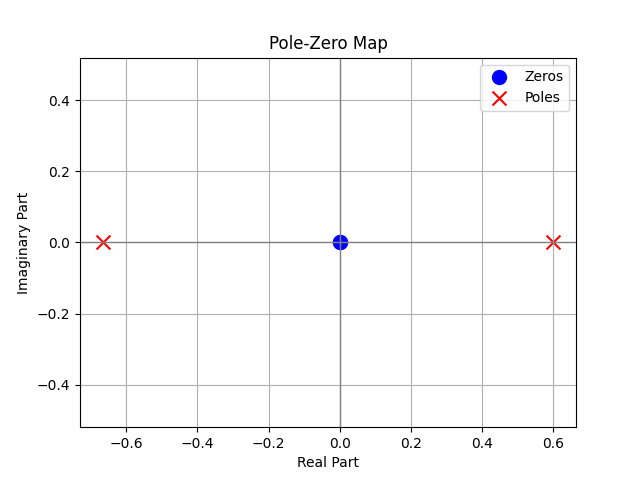
\includegraphics[width=0.8\textwidth]{fig/ex2_d_pole_zero_map.png}
    \caption{Pole-Zero Map of \( H(z) \)}
    \label{fig:ex2_d_pole_zero_map}
\end{figure}

The region of convergence (ROC) for a causal system is outside the outermost pole.

\subsection*{Conclusion}
The poles of the transfer function \( H(z) \) are at \( z = \frac{3}{5} \) and \( z = -\frac{2}{3} \), and the zeros are at \( z = 0 \). The pole-zero map illustrates these locations, and the ROC for a causal system is outside the outermost pole.
